% THIS IS SIGPROC-SP.TEX - VERSION 3.1
% WORKS WITH V3.2SP OF ACM_PROC_ARTICLE-SP.CLS
% APRIL 2009
%
% It is an example file showing how to use the 'acm_proc_article-sp.cls' V3.2SP
% LaTeX2e document class file for Conference Proceedings submissions.
% ----------------------------------------------------------------------------------------------------------------
% This .tex file (and associated .cls V3.2SP) *DOES NOT* produce:
%       1) The Permission Statement
%       2) The Conference (location) Info information
%       3) The Copyright Line with ACM data
%       4) Page numbering
% ---------------------------------------------------------------------------------------------------------------
% It is an example which *does* use the .bib file (from which the .bbl file
% is produced).
% REMEMBER HOWEVER: After having produced the .bbl file,
% and prior to final submission,
% you need to 'insert'  your .bbl file into your source .tex file so as to provide
% ONE 'self-contained' source file.
%
% Questions regarding SIGS should be sent to
% Adrienne Griscti ---> griscti@acm.org
%
% Questions/suggestions regarding the guidelines, .tex and .cls files, etc. to
% Gerald Murray ---> murray@hq.acm.org
%
% For tracking purposes - this is V3.1SP - APRIL 2009

\documentclass{acm_proc_article-sp}

\begin{document}

\title{CS21120: Data Structures and Algorithm Analysis - \\
Sorting}
\subtitle{[Extended Abstract]}
%
% You need the command \numberofauthors to handle the 'placement
% and alignment' of the authors beneath the title.
%
% For aesthetic reasons, we recommend 'three authors at a time'
% i.e. three 'name/affiliation blocks' be placed beneath the title.
%
% NOTE: You are NOT restricted in how many 'rows' of
% "name/affiliations" may appear. We just ask that you restrict
% the number of 'columns' to three.
%
% Because of the available 'opening page real-estate'
% we ask you to refrain from putting more than six authors
% (two rows with three columns) beneath the article title.
% More than six makes the first-page appear very cluttered indeed.
%
% Use the \alignauthor commands to handle the names
% and affiliations for an 'aesthetic maximum' of six authors.
% Add names, affiliations, addresses for
% the seventh etc. author(s) as the argument for the
% \additionalauthors command.
% These 'additional authors' will be output/set for you
% without further effort on your part as the last section in
% the body of your article BEFORE References or any Appendices.

\numberofauthors{1} %  in this sample file, there are a *total*
% of EIGHT authors. SIX appear on the 'first-page' (for formatting
% reasons) and the remaining two appear in the \additionalauthors section.
%
\author{
% You can go ahead and credit any number of authors here,
% e.g. one 'row of three' or two rows (consisting of one row of three
% and a second row of one, two or three).
%
% The command \alignauthor (no curly braces needed) should
% precede each author name, affiliation/snail-mail address and
% e-mail address. Additionally, tag each line of
% affiliation/address with \affaddr, and tag the
% e-mail address with \email.
%
% 1st. author
\alignauthor
James Euesden\\
       \affaddr{Computer Science Department}\\
       \affaddr{Aberystwyth University}\\
       \affaddr{Llandinum Bldg, Penglais}\\
       \affaddr{ Aberystwyth, Dyfed}\\
       \affaddr{SY23 3DB}
       \email{jee22@aber.ac.uk}
}

\maketitle
\begin{abstract}
%%%%%% TO DO!!!!!!!!!
This paper concerns the runtime comparissons of
7 sorting algorithms, that are tried and tested
throughout computer science and software engineering.
The algorithms in question are Bubble, Selection, Insertion,
Shell, Radix, Merge and Quick sort. These are
written and tested in Java. Each algorithm is tested under
similar conditions, and their results are compared to
determine if there are any interesting cross-over points
in their runtimes, and if there is a 'best suited' algorithm.
\end{abstract}

% A category with the (minimum) three required fields
\category{F.2}{ANALYSIS OF ALGORITHMS AND PROBLEM COMPLEXITY}{Nonnumerical Algorithms and Problems}[Sorting and searching]

\terms{Algorithms, Performance}

\keywords{Sorting, Big O} % NOT required for Proceedings

\section{Introduction}
The task set\cite{assignment} was to analyse a minimum of three sorting algorithms,
written in Java, and use each on a number of test samples of data.
These samples of data range from small data sets to very large data
sets, with an initial 13 tests supplied and later extended to 18 tests. 
On each run, the elapsed time from the start of the algorithm to
the completion completion time would be record and compared against
other algorithms in order to reach conclusions.

From the results of the testing, we can compare and contrast each
of the algorithms to determine which are the best for particular
circumstances of varying data set sizes. We will also attempt to 
determine which are the best case average, and examine any particularly 
interesting results and cross-over points between the algorithms 
where one becomes better than another with the different sizes of 
data sets.

The sorting algorithms under test were Bubble Sort, Insertion Sort,
Selection Sort, Shell Sort, Radix Sort, Merge Sort and Quick Sort. For this
report, it is assumed that the reader has a basic knowledge of how these
algorithms work, and a comprehension of their time complexity\cite{complexity}, expressed
in Big O\cite{bigo} notation.

Nowhere in this report will discuss the specifics of what
an algorithm does, or how to write it in code. There are online
resources in the dozens to develop these algorithms, and this report
deals only with their performance in their runtimes and the effect of
different sizes of data sets on each algorithm.


%%%%%%%
\section{The {\secit Body} of The Paper}

\subsection{Materials \& Environment}
In order to get the most accurate and valid results to compare algorithms,
it was necessary to have similar testing conditions for each individual test run.
The environment for all tests was on a Fujitsu Lifebook AH532 Notebook,
running Windows version 8.1 with a 2.6GHz processor and were allowed 
to use up to 3GBs of RAM for each individual test.

All algorithms and the 
testing suite were written in Java, SDK 1.7.0\_51, using 
the IntelliJ IDE for both writing and conducting the tests. All tests were
run under similar conditions, where the device in use was only used for
running the tests and nothing else in order to best
represent each algorithms performance.


%%%%
\subsection{Methods}
To test the sorting algorithms, a testing suite class was written to conduct
single and multiple tests on single and multiple algorithms. Using this class, 
the algorithms were tested multiple times on a total of 18 different data sets,
each with a differing number of items in the set. By testing with many different
varying sizes of data sets, it was possible to see what the effect of the size
of a data set has on the different algorithms, and if some out performed
others on one size, but were outperformed on other sizes, larger or smaller.

These data set sizes ranged from 10 items to 5,000,000 items, and each number contained no more than 6 digits. Some data sets had repeating data, while others did not. These are shown in a table below.

\begin{table}[h]
\centering
\caption{Test files and their data set sizes}
\begin{tabular}{|c|c|l|} \hline
Test Name&Number of items\\ \hline
test1 & 10\\ \hline
test1a & 20\\ \hline
test1b & 50\\ \hline
test2 & 100\\ \hline
test2a & 200\\ \hline
test2b & 500\\ \hline
test3 & 1,000\\ \hline
test3a & 2,000\\ \hline
test3b & 5,000\\ \hline
test4 & 10,000\\ \hline
test4a & 20,000\\ \hline
test4b & 50,000\\ \hline
test5 & 100,000\\ \hline
test5a & 200,000\\ \hline
test5b & 500,000\\ \hline
test6 & 1,000,000\\ \hline
test6a & 2,000,000\\ \hline
test6b & 5,000,000\\ 
\hline\end{tabular}
\end{table}

To get as accurate of a result as possible, each tests runtime was recorded
using nanoseconds, with the Java command \begin{math} System.nanotime() \end{math}.
This was saved to a variable just before the call to begin the sort, and the nanotime was taken again after the completion of the algorithm. This result was then deducted from the start time to result in the elapsed time.
This time was then converted into milliseconds for representation in the spreadsheet of results.

When testing each algorithm on a given data set, the runtime could sometimes be
skewed by the 'warm up' of the processor as it adjusted to the algorithm, or a
result might be abnormal if a sorting process was slowed down due to another process
attempting to use the CPU at the same time. To combat these issues, the
tests were set to run a minimum of 10 times before any elapsed times were recorded,
and treated as  a 'warm up' run for the algorithm,

Once an algorithm had been 'warmed' up on the system, the actual test itereations were run and the elapsed time between
each run was recorded and added to a 'total' time of all runs set for testing. For
the purpose of this task, each algorithm was run on each set of data a total of 100
times. The total time was then divided by the amount of times the test
was run in order to form an average run time. This average run time for each test
is what was considered as the result for each sorting algorithm on each test.

For a number of tests, it was necessary to cancel the sorting part way through, 
or to abort a test entirely. This was based on some tests taking more time than was
reasonable to conclude. These will be discussed in more detail within the
results section.

\subsection{Results}
As each test concluded, the results were stored in a spreadsheet to later
be displayed as line graph for analysis.
Below is a screencap of these results upon completion, where the numbers
shown in the cells are the average runtimes of the algorithm on a particular
amount of items in a data set, displayed in Milliseconds. Those cells where 'DNF' is present 
represent where a test 'Did Not Finish'.

\begin{figure}[h]
\centering
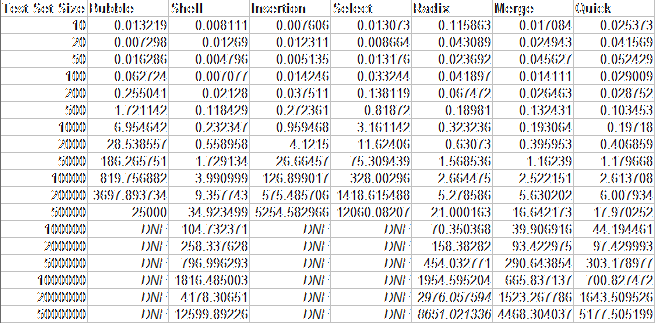
\includegraphics[width=0.48\textwidth]{img/results_table.png}
\caption{The full tests results table}
\end{figure}

As is visible from the results, the simple sorts, Bubble, Insertion and Select,
did not finish or were aborted for the larger test sizes. This was due to the amount of time it began to
take for each sorting algorithm to run the tests. The time it would take became
unreasonable and so it seemed best to abort those tests. Even with not running
these tests, it is apparent from the resulting graph the way in which these  \begin{math}O(n^2)\end{math} time complextity\cite{timec} algorithms
would continue to run and how their results look.

\begin{figure}[h]
\centering
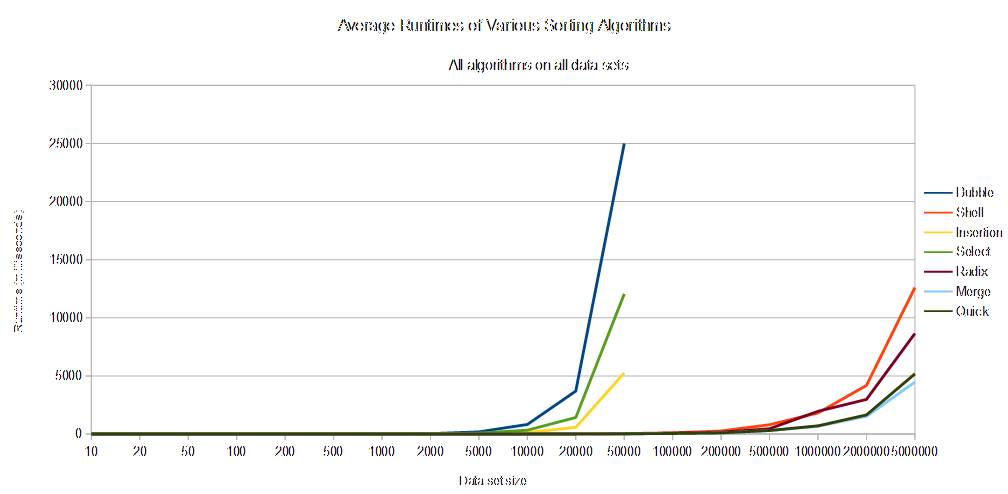
\includegraphics[width=0.48\textwidth]{img/graph_all_tests.png}
\caption{The test results expressed as a line graph}
\end{figure}

This line graph represents the full results contained in the spreadsheet, and stands
as a way of comparing each sorting algorithm against the others. What 
immediately stands out here, is how the simpler algorithms (Bubble, Select, Insertion) begin to take much 
longer than those of \begin{math}O(n log(n))\end{math} and \begin{math}O(nk)\end{math}
 at around the 10,000 items in a data set mark due to their exponential growth rate.

\subsection{Discussion}
To break down the results and intelligently discuss them, the results have been dissected
into more appropriate forms of viewing. To begin, the smaller data (10 - 200) sets were looked at and
analysed to see which sort(s) is the most appropriate for smaller data sets.

\begin{figure}[h]
\centering
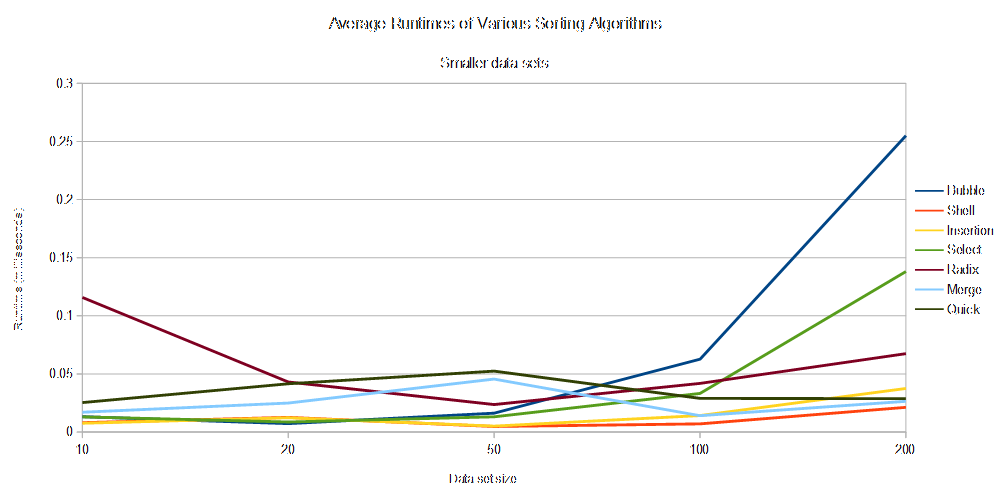
\includegraphics[width=0.48\textwidth]{img/graph_smaller.png}
\caption{Smaller data sets and their results}
\end{figure}

What is most apparent, is that those \begin{math}O(n^2)\end{math} sorting algorithms
that struggle with the larger sets actually out perform the more complicated algorithms
for the data sets below 100-200 items.

Notably, Insertion and Shell sort share very similar time complextities for these smaller 
data sets. As can be seen at the 200 items point though, Shell sort continues
to perform with a lower runtime, while Insertion sort's time begins to break away and 
the algorithm takes longer to iterate through the list. This could be expected, as Shell
sort is based upon Insertion sort, and could be considered as an improvement on Insertion.

At the 200 data set test, it can also be seen that Quick Sort crosses over with the simpler
sorts, beginning to perform at a similar rate as them. With any data sets less than this size,
Quick Sort does not work efficiently compared to the other algorithms. It is in fact one of the 
slowest sorting algorithms for smaller data sets, with Radix sort being the absolute worst 
algorithm until a size of 50 or more items.

\begin{figure}[h]
\centering
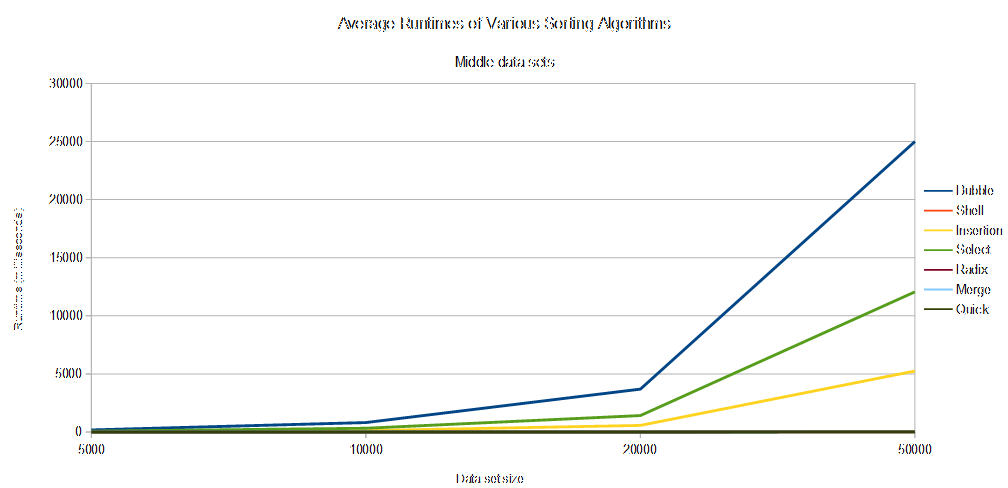
\includegraphics[width=0.48\textwidth]{img/graph_middle.png}
\caption{The data sets from the middle of this reports testing data}
\end{figure}

Another interesting thing to note is how Bubble sort's expoential growth is very visible by
the point there are 100 items of data to process. It is at this stage that the more reliable
algorithms cross over with Bubble sort, and shows why Bubble sort is fine for small data
sets, but terrible when presented with anything moderately large. The same can be said about
Select sort, which also becomes exponentially slower than Bubble sort at 100 items, just
at a lowler rate. This is backed up by when you look at the middle set of data sets tested
for this report.

While the other algorithms continue working at a relatively similar pace, Bubble, Select
and Insertion sort grow exponentially. This leads them up to the tests they did not process, when they were
no longer able to run within a reasonable time frame for the testing. Regardless, it is
relatively easy to predict their expected outcomes for future tests based upon the 
results of the tests that were conducted on these algorithms.

\begin{figure}[h!]
\centering
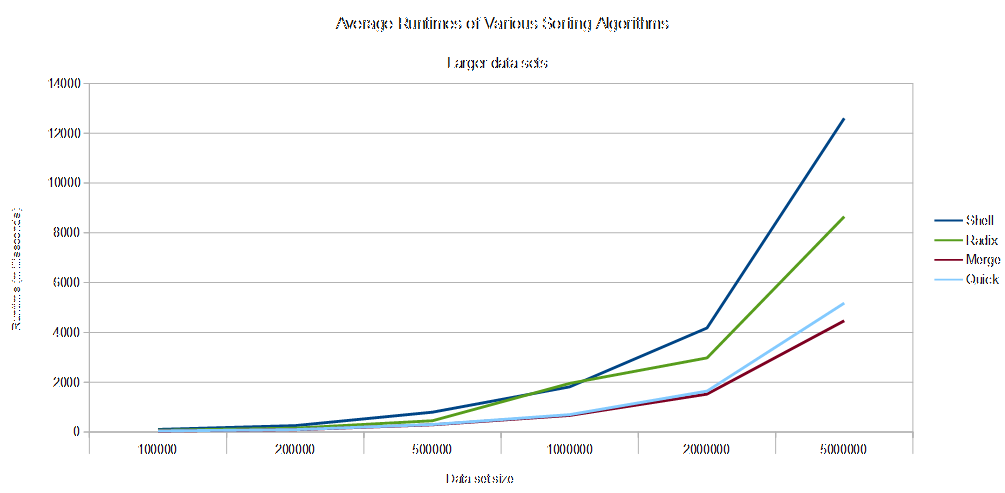
\includegraphics[width=0.48\textwidth]{img/graph_larger.png}
\caption{The larger data sets and test results for applicable algorithms}
\end{figure}

At the other end of the tests, where the data set sizes reach ranges of 100,000 to 5,000,000,
each of the remaining sorting algorithms begins to diverge from each other in their time taken
to sort the items. Merge sort and Quick sort stay very similar to one another with their results,
up until 1,000,000 items. At this point, Quick sort shows itself to be slower at
sorting the data set than Merge sort, although not by much. If more tests on
even greater data sets were to be made, it is probable that we would see Quick sort
progressively slower in it's run time than Merge sort.

As for Radix and Shell sort, while both have up to that point performed similar to
Merge and Quick sort, they both become slower than the others at the 200,000
items in a data set range. Shell sorts 'curve' on the graph becomes a lot steeper,
 a lot faster than Radix sorts does, and we see the point at which it gets incrementally
more difficult for Shell sort to run on larger data sets in comparison to the other algorithms.

A note to make about these tests, with particular attention to Radix sort, is that 
their runtimes and performances will be directly affected by the device they are
run upon. If the device begins to have difficulties in processing such large data
sets, it is very possible that the runtime would be significantly slower than
they would be on a more powerful machine, even if the previous results
were practically identical with smaller data sets on a less powerful machine.

It is for this reason that it may be the curves become so much
steeper so quickly with data sets at this size. However, regardless of the
processing power of the machine and the impact it has upon the runtimes, it
can still be taken as a valid result, since this report is comparing and contrasting
the runtimes of these algorithms against each other. Therefore, these
results can be considered a real life example of a scenario where they are
used on a device requiring them, and which algorithm is still the 'best',
 'worst' and 'average' case, for ranges of data sets, small to large.

This particularily applies to Radix sort, as at the point where it is 
processing sets of items in the million and higher ranges, the space
complexity of the algorithm makes it difficult for some devices to cope with,
resulting in a slower algorithm as the devices RAM is bloated and under strain. This report
still considers this to give an accurate result, based on the 'real world' 
example of how Radix sort compares to the other sorts with the
same working environment.

From analysing and discussing the resulting data from our tests, we can 
see that the 'best sort' for a certain situation can be entirely situational.
For example, it would be foolish to employ a Bubble sort or Selection sort
on a data set larger than 1,000. It is at and after these points 
that these algorithms become the worst to use for their time complexity.

However, if presented with a much smaller size of items, such as one under
200, it would be acceptable to use Bubble or Selection sort over Quick and Merge sort
, although most likely preferable to implement Shell or Insertion sort, as
they handle these smaller data sets better than any other algorithm tested, as seen in the results.

At around the 50,000 items mark, there is a cross over point where it can safely
be said that the size of the data set truly does make a difference. The
simpler algorithms (Selection, Insertion, Bubble) runtime grow at such
an exponential rate that it becomes pointless to use them. While previously,
Quick, Merge and Radix sort were the worst case use for smaller data sets
are now the much more time efficient options.

From this we could conclude that the
runtimes of each algorithm are directly connected to different sizes of
data sets, and some algorithms handle different sizes of data sets much
better (or worse) than others. This is not to say that one should never
use a Quick sort on a smaller data set, however. In fact, it is potentially
the best general purpose sort.

When analysing the results of the smaller data sets below 1000, the difference in 
the runtime between all of the algorithms is rather minimal, and Quick
sort does not perform terribly. Assuming that the algorithms will not
be run on a large quantity of smaller data sets, there would most 
likely not be too much of a noticable difference in performance of
an application.

In the chance that this is the case though, multiple algorithms could be
employed through the use of conditional statements. For example,
when the data set is passed to the application, an if statement
could check and see the size of the data set. If it is greater than
100, then Quick sort may be applied. Otherwise, Insertion sort
could be. This has often been the case with Quick sort in other
applications, using the best algorithm for the task at hand dynamically.
 For testing purpose, however, I felt it best to keep
the two tested individually.

The question may be raised, "Why not say the best average is 
Merge Sort? Which did just as well, if not better, than Quick sort?".
The answer to this is not in the time complexity, but in the space
complexity. Merge sort uses more memory than Quick sort does.

While Quick sort sorts items in-place, using only the original list
of items provided and indexes to where to sort the items, 
Merge sort requires another array in order to separate and 
'merge' the data to be processed.

Unless the device the
 sorting algorithm is running on has enough memory to
 handle this, Quick sort is the better choice for the best average
case sorting algorithm. Plus, as previously stated, it's drawback
with smaller data sets can be overcome with a conditional statement
that processes smaller data sets with Insertion sort.

\section{Conclusions}

The overall conclusion to take from these results are that the
size of a data set directly corresponds to the runtime performance of
an algorithm, and that no one algorithm is best suited for every
single data set, but there is an average best case in QuickSort, 
should an 'all-round' algorithm be required with little specification.

A developer 
should be aware of the differences in run time between the different types
of algorithms and therefore selective of the algorithm they choose to implement 
when using sorting in an application. They should select based upon their 
expected data set sizes, their space requirements and be prepared
to have conditional statements to choose the best algorithm for 
a problem presented to the application.

%\end{document}  % This is where a 'short' article might terminate



%
% The following two commands are all you need in the
% initial runs of your .tex file to
% produce the bibliography for the citations in your paper.
%\bibliographystyle{abbrv}
%\bibliography{sorting_algorithms}  % sigproc.bib is the name of the Bibliography in this case
% You must have a proper ".bib" file
%  and remember to run:
% latex bibtex latex latex
% to resolve all references
%
% ACM needs 'a single self-contained file'!
%
%APPENDICES are optional
%\balancecolumns

\begin{thebibliography}{1}

\bibitem{assignment} R. C. Shipman, {\em "CS21120: Data Structures and Algorithm Analysis Assignment 2 - Sorting}, 25th February 2014.

\bibitem{complexity}
Big-O Algorithm Complexity Cheat Sheet [webpage]. Available: http://bigocheatsheet.com/ Accessed: 12/03/14

\bibitem{bigo}
Big O notation - Wikipedia, the free encyclopedia [webpage]. Available: http://en.wikipedia.org/wiki/Big\_O\_notation Accessed: 12/03/14

\bibitem{timec}
Time complexity - Wikipedia, the free encyclopedia [webpage]. Available: http://en.wikipedia.org/wiki/Time\_complexity Accessed: 12/03/14

\end{thebibliography}

\appendix
%Appendix A
\subsection{Introduction}
\subsection{The Body of the Paper}
\subsubsection{Environment \& Tools}
\subsubsection{Methods}
\subsubsection{Results}
\subsubsection{Discussion}
\subsection{Conclusions}
\subsection{References}


\section{Executive Summary}
\subsection{Mission Statement}
To test the runtimes of different sorting algorithms on data sets of small and large
sizes  to see the performance of each algorithm and analyse the results using line graphs and discussion.
\subsection{Methods}
Testing the algorithms using averaged time recorded in nanoseconds on a
singular device under similar circumstances for multiple tests and iterations. Recording the averaged run time results in a spreadsheet for analysis.
\subsection{Outcomes}
Concluding that the runtime of a sorting algorithm is affected by the size of a
data set and that some algorithms are best suited for larger amounts of sets but bad
for smaller sizes, and visa versa. Determining which algorithm could be best suited
as a 'best average case' sorting algorithm when presented with any size of data set.
\begin{figure*}
\centering
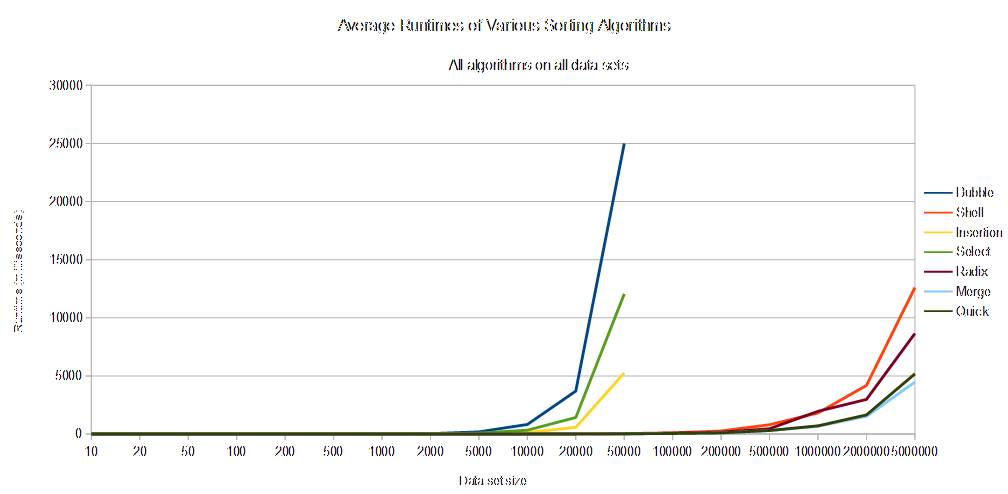
\includegraphics[width=0.7\textwidth]{img/graph_all_tests.png}
\caption{The test results expressed as a line graph}

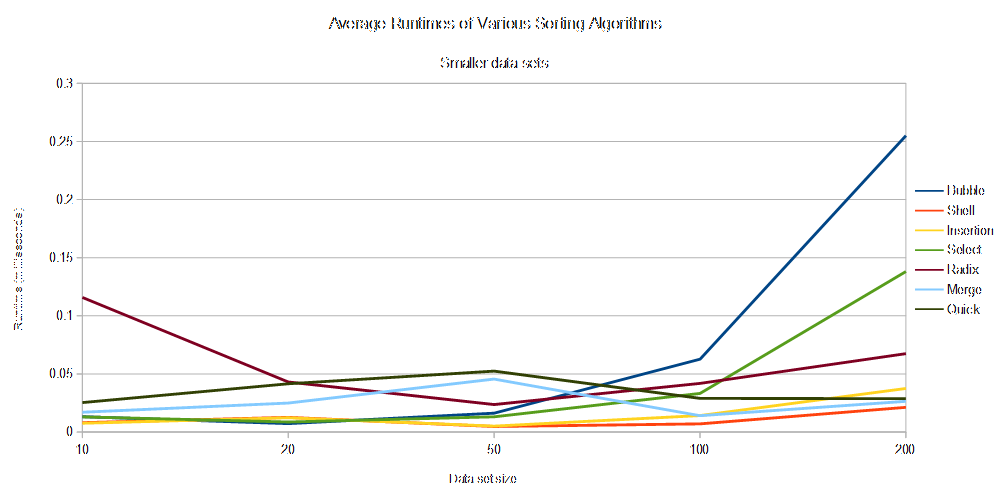
\includegraphics[width=0.7\textwidth]{img/graph_smaller.png}
\caption{Smaller data sets and their results}

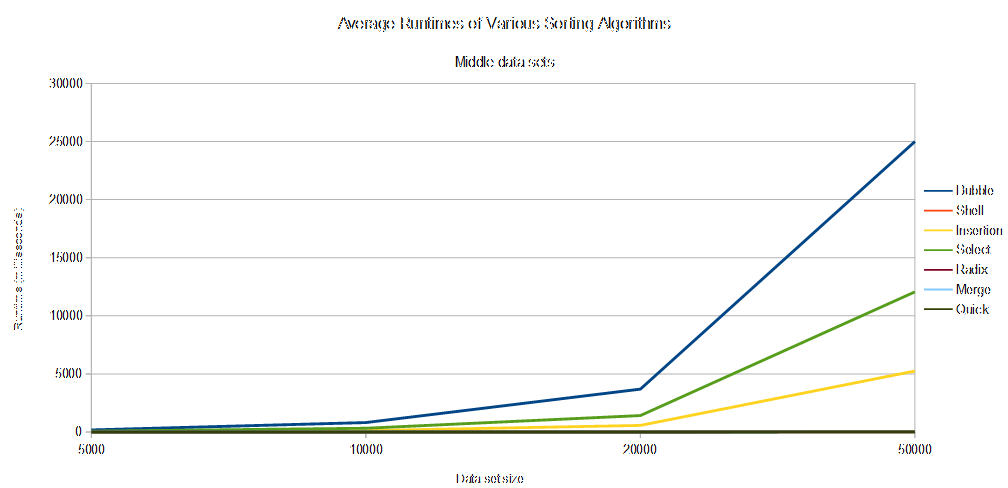
\includegraphics[width=0.7\textwidth]{img/graph_middle.png}
\caption{The data sets from the middle of this reports testing data}

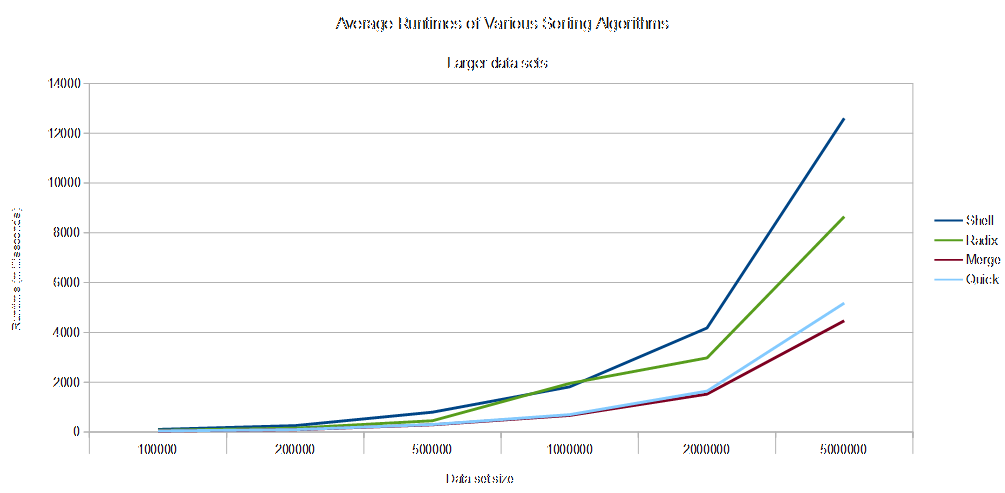
\includegraphics[width=0.7\textwidth]{img/graph_larger.png}
\caption{The larger data sets and test results for applicable algorithms}
\end{figure*}

\balancecolumns
\clearpage
% That's all folks!
\end{document}
